\documentclass[border=2pt]{standalone}
\usepackage{pgfplots}

\begin{document}
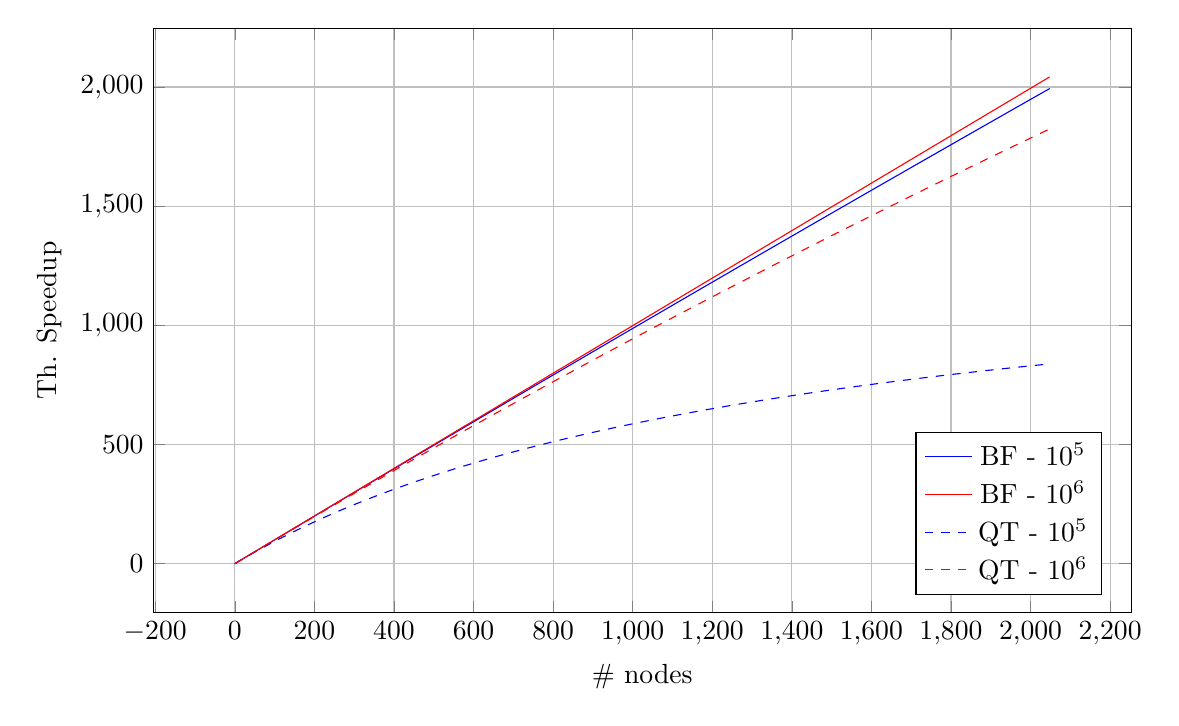
\begin{tikzpicture}
  \begin{axis}[
      xlabel= \# nodes,
      ylabel = Th. Speedup,
      ylabel style={rotate=0},
      width=14cm,
      height=9cm,
      grid=major,
      scaled x ticks = false,
      legend entries={BF - $10^5$, BF - $10^6$, QT - $10^5$, QT - $10^6$},
      legend pos = south east,
      tick label style={/pgf/number format/fixed},
    ]
    \addplot[solid,blue, domain=0:2048, samples=500] {x/(1+(x-1)*0.0000133333)};
    \addplot[solid,red, domain=0:2048, samples=500] {x/(1+(x-1)*0.00000133333)};
    \addplot[dashed,blue, domain=0:2048, samples=500] {x/(1+(x-1)*0.000705)};
    \addplot[dashed,red, domain=0:2048, samples=500] {x/(1+(x-1)*0.00006)};

\end{axis}
\end{tikzpicture}
\end{document}
